
\chapter{TRIỂN KHAI VÀ ĐÁNH GIÁ}\label{section:dev}
\fontsize{13px}{13px}\selectfont\justifying
\section{Triển khai}

\subsection{Cấu hình máy chủ}

\begin{itemize}
	\item \textbf{Máy chủ staging} Virtual CPUs: 1. Memory (RAM): 2048 MB. Disk: 15 GB
	
	\item \textbf{Máy chủ production}. Virtual CPUs: 1. Memory (RAM): 1536 MB. Disk: 15 GB
	
	\item \textbf{Máy chủ database}. Virtual CPUs: 1. Memory (RAM): 1536 MB. Disk: 15 GB
	
	\item \textbf{Máy chủ proxy}. Virtual CPUs: 1. Memory (RAM): 1536 MB. Disk: 15 GB
\end{itemize}
\subsection{Cài đặt tiến trình}


\subsubsection{Máy chủ staging}
\begin{itemize}
	\item Tiến trình accounts chạy ở chế độ staging kết nối với database test
	\item Tiến trình sellers chạy ở chế độ staging kết nối với database test
	\item Tiến trình bloggers chạy ở chế độ staging kết nối với database test
	\item Tiến trình gateway chạy ở chế độ staging cung cấp giao diện quản lí mà sanbox để kiểm tra API.
\end{itemize}
\subsubsection{Máy chủ production}
\begin{itemize}
	\item Tiến trình accounts chạy ở chế độ \emph{production} kết nối với database account
	\item Tiến trình  chạy ở chế độ \emph{production} kết nối với database seller
	\item Tiến trình bloggers chạy ở chế độ \emph{production} kết nối với database blogger
	\item Tiến trình gateway chạy ở chế độ \emph{production} cung cấp giao diện quản lí.
\end{itemize}

\subsubsection{Máy chủ database}
Cấu hình mongodb và cung cấp các database cho các môi trường phát hành.
\begin{itemize}
	\item account
	\item seller
	\item blogger
	\item test (cho môi trường staging)
\end{itemize}
\subsubsection{Máy chủ proxy}
Cấu hình liên kết tên miền với cổng tiến trình của các máy chủ trong hệ thống. Đăng ký chứng thực SSL. Sử dụng các thuật toán cân bằng tải có sẵn để điều phối request.

\FloatBarrier
\begin{figure}[!htbp]\fontsize{13px}{13px}\selectfont
	\begin{center}	
		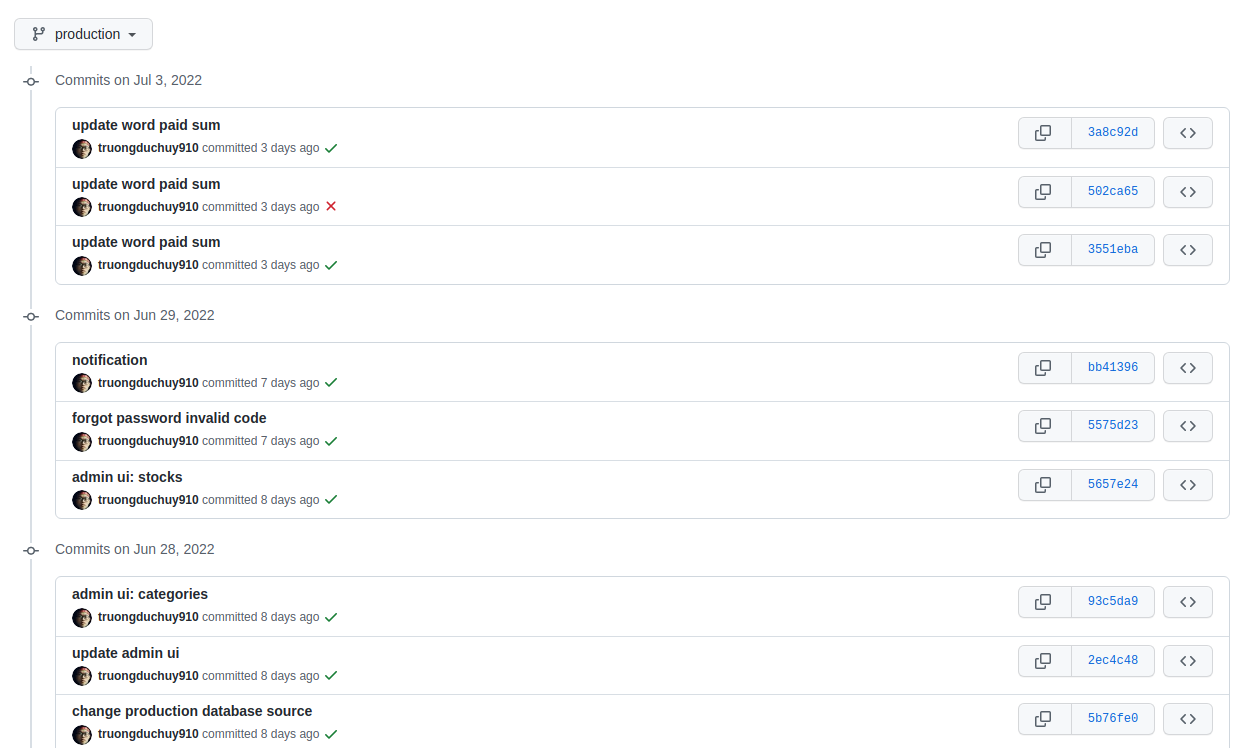
\includegraphics[width=\textwidth]{./results/commit}
		\caption{Lịch sử các phiên bản phát hành môi trường production.}
	\end{center}
	
\end{figure}
\clearpage
\FloatBarrier
\begin{figure}[!htbp]\fontsize{13px}{13px}\selectfont
	\begin{center}	
		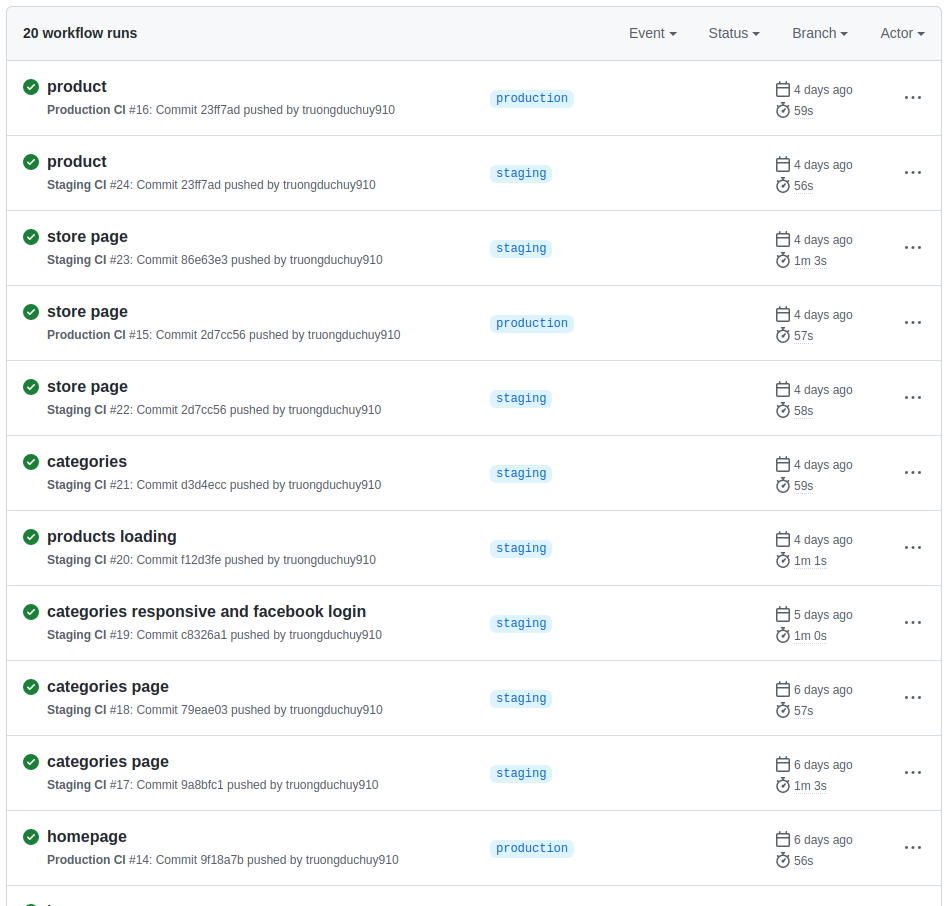
\includegraphics[width=\textwidth]{./results/deployments}
		\caption{Lịch sử cài đặt tiến trình ở các môi trường staging và production sử dụng CI/CD của github actions.}
	\end{center}
	
\end{figure}
\clearpage
\begin{figure}[h!]\fontsize{13px}{13px}\selectfont
	\begin{center}	
		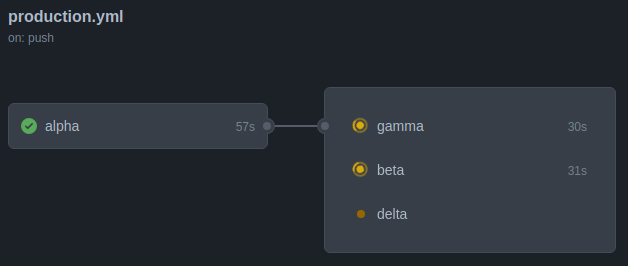
\includegraphics[width=\textwidth]{./results/jobs}
		\caption{Thông tin chi tiết khi sử dụng CI/CD chạy các bản sao của micro service trên nhiều máy chủ khác nhau}
	\end{center}
\end{figure}


\begin{figure}[h!]\fontsize{13px}{13px}\selectfont
	\begin{center}	
		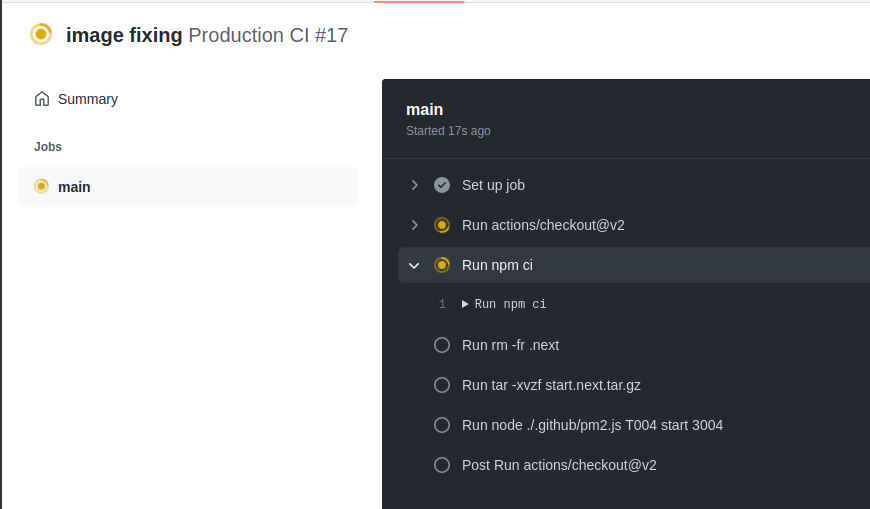
\includegraphics[width=\textwidth]{./results/production}
		\caption{Thông tin chi tiết các bước của một mirco-service sử dụng CI/CD}
	\end{center}
\end{figure}


